\documentclass[english,man]{apa6}
\usepackage{lmodern}
\usepackage{amssymb,amsmath}
\usepackage{ifxetex,ifluatex}
\usepackage{fixltx2e} % provides \textsubscript
\ifnum 0\ifxetex 1\fi\ifluatex 1\fi=0 % if pdftex
  \usepackage[T1]{fontenc}
  \usepackage[utf8]{inputenc}
\else % if luatex or xelatex
  \ifxetex
    \usepackage{mathspec}
  \else
    \usepackage{fontspec}
  \fi
  \defaultfontfeatures{Ligatures=TeX,Scale=MatchLowercase}
\fi
% use upquote if available, for straight quotes in verbatim environments
\IfFileExists{upquote.sty}{\usepackage{upquote}}{}
% use microtype if available
\IfFileExists{microtype.sty}{%
\usepackage{microtype}
\UseMicrotypeSet[protrusion]{basicmath} % disable protrusion for tt fonts
}{}
\usepackage[unicode=true]{hyperref}
\hypersetup{
            pdftitle={Automated detections reveal the social information in the changing infant view},
            pdfkeywords={Postural developments, headcam, social information, face detection, pose
detection},
            pdfborder={0 0 0},
            breaklinks=true}
\urlstyle{same}  % don't use monospace font for urls
\ifnum 0\ifxetex 1\fi\ifluatex 1\fi=0 % if pdftex
  \usepackage[shorthands=off,main=english]{babel}
\else
  \usepackage{polyglossia}
  \setmainlanguage[]{english}
\fi
\usepackage{graphicx,grffile}
\makeatletter
\def\maxwidth{\ifdim\Gin@nat@width>\linewidth\linewidth\else\Gin@nat@width\fi}
\def\maxheight{\ifdim\Gin@nat@height>\textheight\textheight\else\Gin@nat@height\fi}
\makeatother
% Scale images if necessary, so that they will not overflow the page
% margins by default, and it is still possible to overwrite the defaults
% using explicit options in \includegraphics[width, height, ...]{}
\setkeys{Gin}{width=\maxwidth,height=\maxheight,keepaspectratio}
\IfFileExists{parskip.sty}{%
\usepackage{parskip}
}{% else
\setlength{\parindent}{0pt}
\setlength{\parskip}{6pt plus 2pt minus 1pt}
}
\setlength{\emergencystretch}{3em}  % prevent overfull lines
\providecommand{\tightlist}{%
  \setlength{\itemsep}{0pt}\setlength{\parskip}{0pt}}
\setcounter{secnumdepth}{0}
% Manuscript styling
\usepackage{upgreek}
\captionsetup{font=singlespacing,justification=justified}

% Table formatting
\usepackage{longtable}
\usepackage{lscape}
% \usepackage[counterclockwise]{rotating}   % Landscape page setup for large tables
\usepackage{multirow}		% Table styling
\usepackage{tabularx}		% Control Column width
\usepackage[flushleft]{threeparttable}	% Allows for three part tables with a specified notes section
\usepackage{threeparttablex}            % Lets threeparttable work with longtable

% Create new environments so endfloat can handle them
% \newenvironment{ltable}
%   {\begin{landscape}\begin{center}\begin{threeparttable}}
%   {\end{threeparttable}\end{center}\end{landscape}}
\newenvironment{lltable}{\begin{landscape}\begin{center}\begin{ThreePartTable}}{\end{ThreePartTable}\end{center}\end{landscape}}

% Enables adjusting longtable caption width to table width
% Solution found at http://golatex.de/longtable-mit-caption-so-breit-wie-die-tabelle-t15767.html
\makeatletter
\newcommand\LastLTentrywidth{1em}
\newlength\longtablewidth
\setlength{\longtablewidth}{1in}
\newcommand{\getlongtablewidth}{\begingroup \ifcsname LT@\roman{LT@tables}\endcsname \global\longtablewidth=0pt \renewcommand{\LT@entry}[2]{\global\advance\longtablewidth by ##2\relax\gdef\LastLTentrywidth{##2}}\@nameuse{LT@\roman{LT@tables}} \fi \endgroup}

% \setlength{\parindent}{0.5in}
% \setlength{\parskip}{0pt plus 0pt minus 0pt}

% \usepackage{etoolbox}
\makeatletter
\patchcmd{\HyOrg@maketitle}
  {\section{\normalfont\normalsize\abstractname}}
  {\section*{\normalfont\normalsize\abstractname}}
  {}{\typeout{Failed to patch abstract.}}
\makeatother
\shorttitle{Automated detection of social information}
\author{Bria L. Long\textsuperscript{1}, Alessandro Sanchez\textsuperscript{1}, Allison M. Kraus\textsuperscript{1}, Ketan Agrawal\textsuperscript{1}, \& Michael C. Frank\textsuperscript{1}}
\affiliation{
\vspace{0.5cm}
\textsuperscript{1} Department of Psychology, Stanford University}
\authornote{

Correspondence concerning this article should be addressed to Bria L. Long, 450 Serra Mall, Stanford CA 94305. E-mail: bria@stanford.edu}
\keywords{Postural developments, headcam, social information, face detection, pose detection\newline\indent Word count: 7324}
\DeclareDelayedFloatFlavor{ThreePartTable}{table}
\DeclareDelayedFloatFlavor{lltable}{table}
\DeclareDelayedFloatFlavor*{longtable}{table}
\makeatletter
\renewcommand{\efloat@iwrite}[1]{\immediate\expandafter\protected@write\csname efloat@post#1\endcsname{}}
\makeatother
\usepackage{csquotes}

\title{Automated detections reveal the social information in the changing
infant view}

\date{}

\abstract{
•We provided a open, annotated dataset of naturalistic parent-child
interactions during a play session with with novel and familiar toys,
recording the egocentric and third-person views.

•We develop a novel method using a pose detection model to automatically
quantify the faces and hands in the infant view.

•We apply our novel method to this and another egoecentric video
dataset, and confirm that locomotive developments around the first
birthday shape the faces and hands that infants see in naturalistic
interactions.

•The combined use of head-mounted cameras and automated analyses has the
potential to reveal the changing statistics of the information in the
infant view.

Social information plays a key role in infants' early linguistic and
cognitive development. Yet infants locomotor abilities also develop
continuously as they learn to sit, crawl, stand, and walk. How do these
postural developments affect infants access to the social information
relevant for early learning? To address this question, we first created
a rich annotated dataset of naturalistic play sessions between infants
and their caregivers with sets of novel and familiar toys (N=36, 8-16
month-olds), recording both egocentric and third-person video. We then
developed an automated analysis method using a pose detection model to
detect the faces and hands in the infant view. We found that infants'
posture and orientation to their caregiver changed dramatically across
this age range and modulated infants access to social information;
infants who were sitting or standing with their caregiver at a close
distance tended to have the most faces and hands in their visual field.
We applied this automated method to a second egocentric video dataset
from a previous study, replicating and extending their findings on the
influence of infants' posture on the social information in view.
Together, these results establish the validity of a new method for
detecting social information in egocentric videos and confirm that
motoric developments play a significant role in shaping the social
information that infants have access to. The combined use of
head-mounted cameras and new computer vision techniques is a promising
avenue for understanding how the statistics of infants' visual and
linguistic experience change over development.
}

\begin{document}
\maketitle

From their earliest months, infants are deeply engaged in learning from
others. Even newborns tend to prefer to look at faces with direct
vs.~averted gaze (Farroni, Csibra, Simion, \& Johnson, 2002) and young
infants follow overt gaze shifts (Bruner, 1975; Gredeback, Fikke, \&
Melinder, 2010). And as infants reach their first birthday, they also
tend to follow (Yu \& Smith, 2013, 2017) and imitate the gestures of
their caregivers (e.g., pointing). Infants ability to process these
social cues may provide strong scaffolding for early word learning.
Longitudinal studies provide some evidence for this link: children's
level of joint engagement with their mother at 9-12 months predicts both
their receptive and productive vocabularies (Carpenter, Nagell, \&
Tomasello, 1998) and 10 month-olds who follow an adult's gaze (in an
experimental context) have larger vocabularies at 18 months and
throughout the second year of life (Brooks \& Meltzoff, 2005, 2008).
While the relationship between hand-following and language development
has been less well characterized, infants who follow their caregivers'
hands tend to be those who spend more time jointly attending to events
with their caregivers (Yu \& Smith, 2017).

Relatively little work, however, has quantified how often infants see
and use these kinds of social cues in naturalistic learning
environments. By using head-mounted cameras to record what infants see,
researchers have begun to document the infant egocentric perspective
(Yoshida \& Smith, 2008) and to quantify the information -- social and
otherwise -- available to infants as they learn. While head-mounted
camera data do not provide explicit information on where infants are
attending, some work suggests that infants orient their head towards
what they are focusing on -- putting those people or objects in view
(Yoshida \& Smith, 2008). Initial recordings using this technique during
in-lab play sessions revealed a different view than many imagined:
instead of being dominated by faces, the infant perspective contained
close up views of primarily toys and hands (Franchak, Kretch, Soska, \&
Adolph, 2011; Yoshida \& Smith, 2008; Yu \& Smith, 2017). Subsequent
research has revealed that the infant view undergoes dramatic changes as
infants grow. Recordings from home environments suggest that the
viewpoints of very young infants -- less than 4 months of age -- do
indeed contain persistent and frequent views of faces (Fausey,
Jayaraman, \& Smith, 2016; Jayaraman, Fausey, \& Smith, 2017) but that
the infant view tends to contain more and more hands as infants grow
older.

These changes in perspective are likely the downstream consequence of
myriad factors, chief of which may be infants' evolving locomotive
abilities: an infant's ability to sit, crawl, stand, or walk structures
the way they interact with the things and people in their world.
Infants' locomotive abilities can change rapidly: the physical body of
an infant can lengthen up to 2cm in 24 hours (Lampl, 1993), leading to
changes in their abilities from one day to the next. These motoric
developments can be thought of as gateways that open up entirely new
phases of development (Iverson, 2010), causing a cascade of changes in
an infant's ability to interact with their world and the people in it
(Karasik, Tamis-LeMonda, \& Adolph, 2014). Thus, infants' changing
locomotor abilities may shape the social cues that infants' see and seek
out, in turn impacting their cognitive and linguistic abilities.

However, understanding the nuanced relationship between the social
information in the infant view and their motoric and linguistic
development has remained challenging. For example, as children begin
crawling (Adolph, Vereijken, \& Denny, 1998) -- or scooting or cruising
(Patrick, Noah, \& Yang, 2012) -- they are no longer constrained to the
same spot that their caregivers last placed them in. Yet while crawlers
can choose where to go and what they see to a much greater degree, they
also appear to spend much of their time in a world populated by floors
and knees; during spontaneous play, toddlers are more likely to look at
the floor while crawling than while walking (Franchak et al., 2011),
when they have full visual access to their environment and the people in
it (Kretch, Franchak, \& Adolph, 2014). Further, infants' experience
with sitting predicts their success at 3D object completion tasks
(Soska, Adolph, \& Johnson, 2010) as well as their receptive vocabulary
(Libertus \& Violi, 2016), suggesting the importance of focused play
sessions for language development.

Others have posited that it is children's ability to stand and walk that
fundamentally changes their ability to access social information (e.g.,
facial expressions, gaze cues, pointing) relative to children who are
still crawling and sitting (Walle, 2016), which in turn allow infants to
learn words quicker and more efficiently (Walle, 2016). Supporting this
idea, walking vs.~crawling infants tend to make different kinds of
object-related bids for attention from their caregivers (Karasik et al.,
2014), hear more action directed statements (e.g., \enquote{open it})
(Karasik et al., 2014), and have higher receptive and productive
vocabularies (Walle \& Campos, 2014). However, not all evidence supports
this view: parental report data suggest a weak relationship between
walking and the onset of language (Moore, Dailey, Garrison, Amatuni, \&
Bergelson, 2019), and head-mounted eye-tracking data from one-year-olds
highlights the role of infants' in-the-moment posture -- and that of
their caregivers' -- in what infants' see, finding that these factors
are better predictors of the social information in view than their
locomotor status per se (i.e., \enquote{walker} vs \enquote{crawler})
(Franchak, Kretch, \& Adolph, 2017).

Broadly, the field is in need of computational tools to reuse these rich
video datasets and understand the generalizability of findings across
different populations, tasks, and age-ranges. For example, different
kinds of play sessions (e.g., exploring novel environments vs.~playing
with novel objects) might modulate the degree to which infants' posture
changes the social information in view. Yet while the field has
assembled many head-mounted camera datasets, conducting new analyses on
these videos has remained prohibitively time-consuming due to a lack of
computational tools for annotations. Instead, hundreds of hours of
manual annotations have been required to analyze a fraction of the
available frames for a given analysis. Thus despite containing a wealth
of information about the structure of parent-child interactions, these
datasets have thus gone dramatically underused.

Recent innovations in computer vision hold promise for automated
annotations of the infant view. Over the past decade, deep neural
networks have become dramatically better at a wide range of visual
tasks, including object classification, Simonyan and Zisserman (2014),
scene categorization (Zhou, Lapedriza, Khosla, Oliva, \& Torralba,
2017), and pose detection (K. Zhang, Zhang, Li, \& Qiao, 2016), arguably
facilitating our understanding of visual perception (Peterson, Abbott,
\& Griffiths, 2018; VanRullen, 2017) and improving computational
neuroscience (Kietzmann, McClure, \& Kriegeskorte, 2018). However, as
most models have been trained on photographs or videos taken from the
adult perspective, it is still unclear how easily these models can be
applied to videos taken from the infant perspective.

In the present paper, we make progress on understanding the relationship
the between the infant visual perspective and motoric and linguistic
development in three ways. First, we validate a model for the automated
detection of faces and hands in the infant view. We use an open-source
model of pose detection -- OpenPose (Cao, Simon, Wei, \& Sheikh, 2017;
K. Zhang et al., 2016) -- that provides pose, face, and hand keypoints
for every person in an image. We compare the detection accuracy of this
method with that of both older and more specialized models of face
detection, and demonstrate the usability of this off-the-shelf model for
quantifying the faces and hands in the infant view.

Second, we provide an annotated, open dataset for researchers to examine
the effects of postural developments and naming behavior during
naturalistic parent-child interactions. To do so, we invited caregivers
of 8, 12, and 16-month-olds to participate in play sessions where they
were provided with pairs of novel and familiar objects (e.g., a ball and
a microfiber duster, called a \enquote{zem}). We chose this age-range to
span the months when infants typically transition from sitting to
crawling to standing, and documented the infant egocentric view as well
as a third-person view of the play session. We then annotated infants'
in-the-moment posture and orientation relative to their caregiver, and
obtained full transcripts of the play sessions as well as
MacArthur-Bates Communicative Development Inventories for each child.

Third, we apply our automated method to this and one other openly
available head-mounted camera dataset, examining the generality of the
effects of motor development on the social information in view. In Study
1, we use the cross-sectional design of our dataset to directly examine
the relative contributions of age vs.~in-the-moment posture on infants'
visual access to social information, and use the transcriptions to
examine how the availability of social cues changes relative to naming
events (e.g., \enquote{Yes, you like the {[}ball!{]}}). Indeed, despite
positing links between the social information in view and language
development, no work to date has directly examined how the availability
of social information changes around naming events in naturalistic
contexts. In Study 2, we apply this automated method to Franchak et al.
(2017), where one-year-olds wore head-mounted eye-tracking cameras
during a play session and their in-the-moment posture was
hand-annotated. Unlike the present dataset, infants and caregivers
roamed a large, open playroom and explored different toys placed
throughout. We thus analyzed this second dataset with a first goal of
validating our automated method on a very different kind of video
dataset, attempting to replicate their primary findings originally
obtained with a head-mounted eye-tracker, and then further examine
whether the proportion of hands in view also varies with infants'
posture. Broadly, we predicted that there would be differential access
to social information based on children's postural developments:
crawling infants would see fewer faces/hands because they would
primarily be looking at the ground, while walking toddlers would have
access to a richer visual landscape with greater access to the social
information in their environment.

\section{Study 1}\label{study-1}

\subsection{Methods}\label{methods}

Caregivers of 8, 12, and 16-month-olds were invited to participate in
play sessions where they were provided with pairs of novel and familiar
objects (e.g., a ball and a microfiber duster, called a \enquote{zem})
in a small playroom in a lab (approximately 10' x 10'). Infants wore
head-mounted cameras equipped with a fish-eye lens (see Head-mounted
camera), a tripod-mounted camera captured a third-person view of the
play session. Using these video data, infants' posture and orientation
to their caregiver were hand-coded and annotated for the entirety of the
play session. All videos were transcribed, and MacArthur CDIs were
collected for all children who participated. All materials have been
made publicly available on Databrary for whom the parents provided
sharing consent (29/36 dyads) via {[}BLINDED{]}.

\subsubsection{Participants}\label{participants}

Our final sample consisted of 36 infants and children, with 12
participants in three age groups: 8 months (6 F), 12 months (7 F), and
16 months (6 F). Participants were recruited from the surrounding
community via state birth records, had no documented disabilities, and
were reported to hear at least 80 percent English at home. Demographics
and exclusion rates are given in the table below (see Table 1).

\begin{table}[ht]
\centering
\begin{tabular}{rrrrrr}
\hline
Group & N & \% incl. & Avg age & Avg video length (min) \\
\hline
8 mo. &   12 & 0.46 & 8.71 & 14.41 \\
12 mo. &  12 & 0.40 & 12.62 & 12.71 \\
16 mo. &  12 & 0.31 & 16.29 & 15.10\\
\hline
\end{tabular}
\caption{Exclusion rates and summary demographics for the infants included in the study.} 
\end{table}

To obtain this final sample, we tested 95 children, excluding 59
children for the following reasons: 20 for technical issues related to
the headcam (e.g., failure to record, ran out of battery), 15 for
failing to wear the headcam, 10 for fewer than 4 minutes of headcam
footage, 5 for having multiple adults present, 5 for missing
Communicative Development Inventory (CDI) data, 2 for missing scene
camera footage, 1 for fussiness, and 1 for sample symmetry.
16-month-olds tolerated the head-mounted camera less well than younger
infants, leading to a higher exclusion rate. All inclusion decisions
were made independent of the results of subsequent analyses.

\subsubsection{Head-mounted camera}\label{head-mounted-camera}

We used a head-mounted camera (\enquote{headcam}) that was constructed
from a small camera attached to a soft elastic headband.\footnote{Detailed
  instructions for creating this headcam can be found at {[}BLINDED{]}.}
Initial participants wore an MD-80 camera, which was then replaced by a
Veho pro camera which had better battery life and a larger view angle.
The view angle of the MD-80 camera was \(32^{\circ}\) horizontal by
\(24^{\circ}\) vertical, and we attached a fish-eye lens to the camera
to increase the view angle to \(64^{\circ}\) horizontal by
\(46^{\circ}\) vertical. The view angle of the Veho pro camera was
wider, \(47^{\circ}\) horizontal by \(36^{\circ}\) vertical. Videos
captured by MD-80/Veho cameras were 640x480/720x480 pixels,
respectively, and both cameras had a frame rate of \textasciitilde{}30
frames per second. To ensure that detections across these different
cameras were comparable, we excluded detections from the outer edges of
the videos taken with the MD-80 cameras based on these view angle
differences in our main analyses (i.e.~excluding top/bottom 13\% of the
frames, and left/right 10\% of the frames).

However, the vertical field of view of the cameras were still
considerably reduced compared to the infants' field of view, which spans
around 100--120\(^{\circ}\) in the vertical dimension by 6-7 months of
age (Cummings, Van Hof-Van Duin, Mayer, Hansen, \& Fulton, 1988; Mayer,
Fulton, \& Cummings, 1988). As we were primarily interested in the
presence of faces in the child's field of view, we chose to orient the
camera upwards to capture the entirety of the child's upper visual field
where the child is likely to see adult faces, understanding that this
decision limited our ability to detect hands (especially those of the
child, which are typically found at the bottom of the visual field). We
note that these limitations regarding field of view and camera angle
affect all studies using this method, not only our own.

\subsubsection{Procedure}\label{procedure}

All parents signed consent documents while children were fitted with the
headcam. If the child was uninterested in wearing the headcam or tried
to take it off, the experimenter presented engaging toys to try to draw
the child's focus away from the headcam. When the child was comfortable
wearing the headcam, the child and caregiver were shown to a playroom
for the free-play session. Parents were shown a box containing three
pairs of familiar and novel objects. These pairs consisted of a ball
paired with a microfiber duster (a \enquote{zem}), a toy car paired with
a cheese grater (a \enquote{manu}), and a brush paired with a back
massager (a \enquote{tima}). Parents were instructed to play with the
object pairs with their child one at a time, \enquote{as they typically
would.}

All parents confirmed that their child had not previously seen the novel
toys and were instructed to use the novel labels to refer to the toys.
The experimenter then left the playroom for approximately 15-20 minutes,
during which a tripod-mounted camera in the corner of the room recorded
the session and the headcam captured video from the child's perspective.

\subsubsection{Data processing and
annotations}\label{data-processing-and-annotations}

Headcam videos were trimmed such that they excluded the instruction
phase when the experimenter was in the room and were automatically
synchronized with the tripod-mounted videos using FinalCut Pro Software.
These sessions yielded 507 minutes (almost a million frames) of video,
with an average video length of 14.07 minutes (min = 4.53, max = 19.35).

\paragraph{Posture and caregiver orientation
annotations}\label{posture-and-caregiver-orientation-annotations}

We created custom annotations to describe the child's physical posture
(i.e.~standing) and the orientation of the caregiver relative to the
child (e.g.~far away). The child's posture was categorized as being
carried, prone (crawling or lying), sitting, or standing. The
caregiver's orientation was characterized as being close, far, or behind
the child (independent of distance). For the first two annotations
(close/far from the child), the caregiver could either be to the front
or side of the child. All annotations were made by a trained coder using
the OpenSHAPA/Datavyu software (Adolph, Gilmore, Freeman, Sanderson, \&
Millman, 2012). Times when the child was out of view of the tripod
camera were marked as uncodable and were excluded from these
annotations; similarily, times when the child was being carried or the
caregivers were out of the frame were marked as uncodable for caregiver
orientation. On average, posture or orientation was uncodable from 1-2
minutes of data in each child (seconds excluded from analysis for
posture, M = 105s, SD = 234s; orientation; M = 105s, SD = 234s), and
these rates did not vary substantially with the age of the child. To
assess the reliability of these annotations, a second coder annotated
videos from three different children to calculate Cohen's kappa
(posture, \(\kappa\) = .82; caregiver orientation, \(\kappa\) = .73).

\paragraph{Naming event annotations}\label{naming-event-annotations}

One coder listened to all of the audio from the play sessions and marked
the exact timestamps whenever one of the novel or familiar objects was
named in any instance (e.g., \enquote{Look at the {[}ball{]}},
\enquote{Can you say {[}zem{]}?}); a second coder listened to the
majority of the play sessions (N = 23 sessions) and also annotated all
naming events. To asesess reliability, we calculated the proportion of
naming events detected by the first coder that were also annotated by
the second coder within a sliding window. We found that 82.1\% of naming
events were detected within a 4 second window (+/- 2s), and 70.9\% of
namings events were detected within a 2 second window (+/- 1s). We also
obtained full text transcriptions of the entire play sessions (with time
stamps marking 10s intervals). While these full transcriptions are not
used in the present analyses, they have been made publically avaliable
for future research.

\subsection{Face and hand detection}\label{face-and-hand-detection}

We evaluated three detection systems for the ability to measure infants'
visual access to faces. The first of these is the most commonly-used and
widely available face detection algorithm: Viola-Jones (Viola \& Jones,
2004). We used this algorithm as a benchmark for performance, as while
it can achieve impressive accuracy in some situations, it is notoriously
bad at dealing with occluded faces (Scheirer, Anthony, Nakayama, \& Cox,
2014). We next tested the performance of two face detectors that both
made use of relatively recently developed Convolutional Neural Networks
(CNNs) to extract face information. The first algorithm was specifically
optimized for face detection, and the second algorithm was optimized to
extract pose information of all the individuals in an image,
operationalized as information about the position of 18 different body
parts. For this second algorithm (OpenPose; Cao et al., 2017), we used
the agent's nose (one of the body keypoints detected) to operationalize
the presence of faces, as any half of a face necessarily contains a
nose.

The OpenPose detector also provided us with the location of an agent's
wrists, which we used as a proxy for hands for two reasons. First, as we
did not capture children's entire visual field, the presence of a wrist
is likely often indicative of the presence of a hand within the field of
view. Second, hands are often occluded by objects when caregivers are
interacting with children, yet still visually accessible by the child
and part of their joint interaction.

\subsubsection{Algorithms}\label{algorithms}

Viola Jones, the first face detection system, made use of a series of
Haar feature-based cascade classifiers (Viola \& Jones, 2004) applied to
each individual frame. The second algorithm (based on work by K. Zhang
et al., 2016) uses multi-task cascaded convolutional neural networks
(MTCNNs) for joint face detection and alignment, built to perform well
in real-world environments where varying illuminations and occlusions
are present. We used a Tensorflow implementation of this algorithm
available at \url{https://github.com/davidsandberg/facenet}.

The CNN-based pose detector (OpenPose; Cao et al., 2017; Simon, Joo,
Matthews, \& Sheikh, 2017; Wei, Ramakrishna, Kanade, \& Sheikh, 2016)
provided the locations of 18 body parts (ears, nose, wrists, etc.) and
is available at
\url{https://github.com/CMU-Perceptual-Computing-Lab/openpose}. The
system uses a convolutional neural network for initial anatomical
detection and subsequently applies part affinity fields for part
association, producing a series of body part candidates. The candidates
are then matched to a single individual and finally assembled into a
pose; here, we only made use of the body parts relevant to the face and
hands (nose and wrists), though the entire set of keypoints is publicly
avaliable. Each keypoint was accompanied by a confidence score made by
the detector.

\subsubsection{Detector evaluation}\label{detector-evaluation}

To evaluate face detector performance, we hand-labeled a \enquote{gold
set} of frames extracted from the video dataset. To account for the
relatively rare appearance of faces in the dataset, we hand-labeled two
types of samples: a sample containing a high density of faces (half
reported by MTCNN, half by OpenPose) and a random sample from the
remaining frames. Each sample was comprised of an equal number of frames
taken from each child's video. For wrist detections, the \enquote{gold
set} was constructed in the same manner, except frames with a high
density of wrists came only from detections made by OpenPose. Faces were
classified as present if at least half of the face was showing; wrists
were classified as present if any part of the wrist was showing. Two
authors labelled the frames independently and resolved disagreements on
a case-by-case basis. Precision (hits / hits + false alarms), recall
(hits / hits + misses), and F-score (harmonic mean of precision and
recall) were calculated for all detectors.

\subsection{Results}\label{results}

First, we report the accuracy of the automated detectors, as assessed by
comparison to hand-labelled frames from the free-play video dataset
described above. We then apply one of these automated detectors
(OpenPose) to the entirety of this video dataset, and use these outputs
to examine how postural developments influence children's visual access
to faces and hands from 8-16 months of age. We further use the
detections to examine how access to these social cues changes during
naming events (e.g., do you see the {[}zem{]}?). Finally, we apply this
same automated detector to another video dataset (Franchak et al.,
2017), replicating and extending their findings on the effects of
posture on visual access to social information.

\begin{figure}[H]
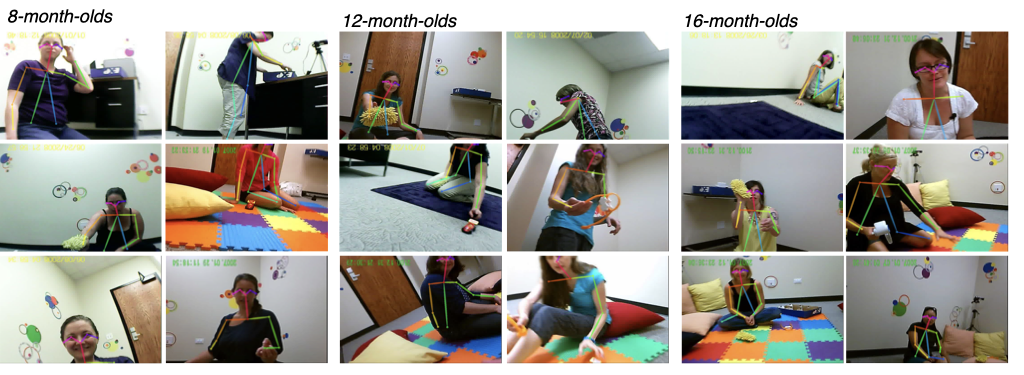
\includegraphics[width=1\linewidth]{images/exampe_detections} \caption{Example detections made by OpenPose from children in each age group.}\label{fig:exampledetections}
\end{figure}

\subsubsection{Accuracy of automated
detections}\label{accuracy-of-automated-detections}

For face detection, we found that both OpenPose and MTCNN dramatically
outperformed ViolaJones (our baseline model) especially with respect to
the random sample, where ViolaJones missed many face that were in view
(see Table 1). When considering only the composite F-score across all
frames, MTCNN slightly outperformed OpenPose (0.89 MTCNN vs.~0.83
OpenPose), and MTCNN and OpenPose performed comparably with the random
sample. Generally, MTCNN exhibited higher precision, whereas OpenPose
exhibited higher recall, and these differences were most pronounced on
the randomly sample frames. In other words, while OpenPose generated
slightly more false positives than MTCNN, MTCNN missed several faces
that were accurately detected by OpenPose. When we restricted our
analysis to high-confidence detections from OpenPose (\textgreater{}.5
confidence; default threshold for visualization), we found very high
precision (P = 0.97), but much lower recall (R = 0.64) and thus overall
lower performance (F = 0.77), indicating that these low-confidence
detections often indexed actual faces that were in the infant view.
Figure \ref{fig:exampledetections} shows example successful detections
from OpenPose in each age group, and Figure \ref{fig:failures} shows
examples of missed faces as well as false positives for context.

We next assessed the viability of OpenPose as a hand detector. Despite
the fact that hand detection is a more computationally challenging
problem (Bambach, Crandall, Smith, \& Yu, 2017), and the fact that we
used wrist keypoints as a proxy for hands, OpenPose performed moderately
well as a hand detector (F = 0.73). OpenPose achieved relatively high
precision -- generating relatively few false positives -- but showed low
recall on the randomly sampled frames (see Table 1). As with face
detections, when we restricted our analysis to high-confidence
detections, we found much higher precision (P = 0.95), but much lower
recall (R = 0.36) and thus lower overall performance (F = 0.52).

Thus, one major advantage of OpenPose relative to specialized face
detectors, such as MTCNN, is that it allows the analysis of both the
faces and hands in the infant view with the outputs of only one
algorithm, and analyzing the results of all detections (regardless of
confidence) yielded reasonably accurate results. Going forward, we
analyze face and wrist detections using all detections from OpenPose,
with the caveat that we are likely underestimating the proportion of
hands in the dataset given the lower recall for hand detections.

\begin{figure}[H]
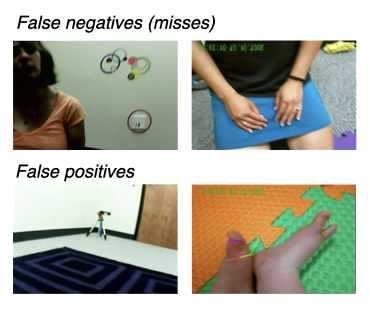
\includegraphics[width=0.5\linewidth]{images/example_failures} \caption{Example failed detections from OpenPose, showing both false positives and false negatives (i.e. missed detections).}\label{fig:failures}
\end{figure}

\begin{table}[ht]
\centering
\begin{tabular}{llrrr}
  \hline
Algorithm & Sample\ Type & P & R & F \\ 
  \hline
MTCNN-Faces & High density & 0.89 & 0.92 & 0.90 \\ 
  MTCNN-Faces & Random & 0.94 & 0.62 & 0.75 \\ 
  OpenPose-Faces & High density & 0.78 & 0.93 & 0.84 \\ 
  OpenPose-Faces & Random & 0.72 & 0.80 & 0.76 \\ 
  OpenPose-Faces-Strict & High density & 0.97 & 0.65 & 0.78 \\ 
  OpenPose-Faces-Strict & Random & 0.97 & 0.62 & 0.76 \\ 
  ViolaJones-Faces & High density & 0.96 & 0.44 & 0.60 \\ 
  ViolaJones-Faces & Random & 0.44 & 0.38 & 0.41 \\ 
  \hline
  \hline
  OpenPose-Wrists & High density & 0.66 & 0.96 & 0.78 \\ 
  OpenPose-Wrists & Random & 0.88 & 0.29 & 0.43 \\ 
  OpenPose-Wrists-Strict & High density & 0.95 & 0.44 & 0.60 \\ 
  OpenPose-Wrists-Strict & Random & 1.00 & 0.10 & 0.18 \\
   \hline
\end{tabular}
\caption{Detector performance on both high density samples (where proportion of targets detected was high) and random samples (where frames were randomly selected). P, R, and F denote precision, recall, and F-score, respectively. "Strict" denotes when we only considered high confidence detections.} 
\vspace{-1em}
\end{table}

\begin{figure}[H]
\includegraphics[width=\textwidth]{figs/posture-1} \caption{Proportion of time spent by each infant in different postures and orientations relative to their caregivers (CG); times where posture was not codable are ommitted for visualization purposes}\label{fig:posture}
\end{figure}

\begin{figure}[H]
\includegraphics[width=\textwidth]{figs/indivPosOrient-1} \caption{Proportion of time spent by each infant in different postures and orientations relative to their caregivers (CG); times when infant was carried or when posture/orientation were not codable are ommitted for visualization purposes}\label{fig:indivPosOrient}
\end{figure}

\subsubsection{Developmental changes in infant posture and caregiver
orientation}\label{developmental-changes-in-infant-posture-and-caregiver-orientation}

Consistent with previous literature (Adolph \& Berger, 2006), the
proportion of time infants spent sitting decreased with age, and the
proportion of time infants spent standing increased with infants' age.
As children got older, their locomotor abilities allowed them to become
more independent. Both 8-month-olds and 12-month-olds spent relatively
equivalent amounts of time lying/crawling (i.e., \enquote{prone}) which
was markedly decreased in the 16-month-olds, who spent most of their
time sitting or standing (see Figure \ref{fig:posture}). We also
observed changes in infants' orientation relative to their caregivers:
the 8-month-olds spent more time with their caregiver behind them
supporting their sitting positions than did children at other ages (see
Figure \ref{fig:posture}). However, we also saw considerable variability
across children: some infants spent almost their entire time sitting at
a close distance from their caregiver, whereas others showed more
considerable variability (see Figure \ref{fig:indivPosOrient}).

\subsubsection{Changes in access to faces and
hands}\label{changes-in-access-to-faces-and-hands}

First, we examined the proportion of face and hand detections as a
function of infants' age without considering their posture (see Figure
\ref{fig:detByAge}). While faces tended to be in the field-of-view
overall more often than hands, infants' head-mounted cameras were angled
slightly upward to capture the presence of faces, and hand detections
suffered from somewhat lower recall than face detections. We thus only
considered differences in the relative proportion of faces or hands in
view as a function of age, posture, and orientation, rather than
comparing them directly. Overall, we did not observe strong age related
trends from 8-16 months of age; if anything, face detections showed a
slight u-shaped pattern, with 12-month-olds having slightly fewer faces
in their visual field that 8- or 16-month-olds.

\begin{figure}[H]
\includegraphics[width=\textwidth]{figs/detByAge-1} \caption{Proportion of faces (left) and wrists (right) detected by the OpenPose model as a function of child's age. Larger dots indicate children who had longer play sessions and thus for whom there was more data.}\label{fig:detByAge}
\end{figure}

\begin{figure}[H]

{\centering \includegraphics[width=\textwidth]{figs/detByPosOrient-1} 

}

\caption{Proportion of face / wrist detections by children's age, their posture, and their caregivers orientation. Data points are scaled by the amount of time spent in each orientation/posture combination; times when posture/orientation annotatinos were unavaliable or the infant was carried are not plotted. Error bars represent 95\% bootstrapped confidence intervals}\label{fig:detByPosOrient}
\end{figure}

In contrast, infant's locomotor developments had a major effect on the
faces and hands that were in the field of view (see Figure
\ref{fig:detByPosOrient}). Two generalized linear mixed-effect models
were used to predict the proportion of faces and hands in view, with
orientation, posture, their interaction, and scaled participant's age as
fixed effects, and with random slopes for infants' orientation and
posture (see all coefficients in Tables 3 and 4). In particular, the
interaction between infants' posture and their caregiver's orientation
had the most dramatic effect on the social information in view. When
caregivers were behind their infants, supporting their infants' sitting
or standing positions, infants saw fewer faces. When caregivers were
relatively close to their infants, infants who were sitting or standing
had more faces in view (Face detections; infant sitting and caregiver
(CG) close, b = 0.90, SE = 0.07, Z = 13.80, P \textless{} 0.001; infant
standing and CG close, b = 1.23, SE = 0.08, Z = 15.44, P \textless{}
0.001) than infants who were lying down/crawling (i.e.~prone). When
caregivers were far away from their infants, face detections were
similarity higher (Face detections; infant sitting and CG far, b = 0.63,
SE = 0.07, Z = 9.16, P \textless{} 0.001; infant standing and CG far, b
= 1.23, SE = 0.09, Z = 14.43,P \textless{} 0.001). Infants' age was not
significant predictor in accounting for the faces in view (Face
detections; Age (scaled), b = 0.04, SE = 0.11, Z = 0.42, P = 0.671).

We found a similar pattern of results for wrist detections, even though
there were fewer wrist detections overall in the dataset. Infants saw
fewer wrists when caregivers were behind their infants, supporting their
infants' sitting or standing positions vs when caregivers were
relatively closer to their infants (Hand detections; infant sitting and
CG close, b=0.27, SE = 0.08, Z = 3.35, P \textless{} 0.001; infant
standing and CG close, b=0.53, SE = 0.09, Z = 6.07, P \textless{} 0.001)
than infants who were lying down/crawling (i.e.~prone). Wrist detections
were highest when caregivers were far away from their infants and those
infants were standing (Wrist detections; infant standing and CG far, b =
1.57, SE = 0.11, Z = 14.16, P \textless{} 0.001). As with faces, age was
not a significant predictor in these models (Wrist detections; Age
(scaled), b = 0.09, SE = 0.11, Z = 0.86, P = 0.390).

We directly examined the contributions of posture and orientation
vs.~age by fitting a reduced version of the full model (Nakagawa \&
Schielzeth, 2013) without their fixed effects (both models were run with
the maximal random effects structure), and comparing model fits for each
of these. The fixed effects in a model with only the age of the
participants accounted for relatively little variance in the proportion
of faces (marginal \(R^2\) \textless{} 0.01) or hands in view (marginal
\(R^2\) = 0.02). However, when adding infants' posture and orientation
to their caregiver to the model (and their interaction) the marginal
\(R^2\) were higher for both faces (marginal \(R^2\) = 0.25) and wrists
(marginal \(R^2\) = 0.26). Overall, these results suggest that infants'
visual access to social information is largely modulated by their
posture and orientation to their caregiver, which is in turn a function
of their general locomotor development.

\begin{table}[ht]
\centering
\begin{tabular}{rrrrr}
  \hline
 & Estimate & Std. Error & z value & Pr($>$$|$z$|$) \\ 
  \hline
Intercept & -3.24 & 0.20 & -16.37 & 0.000 \\ 
  Sit & -0.00 & 0.19 & -0.02 & 0.988 \\ 
  Stand & -0.29 & 0.20 & -1.44 & 0.151 \\ 
  Close & 0.02 & 0.18 & 0.10 & 0.917 \\ 
  Far & 0.51 & 0.25 & 2.04 & 0.041 \\ 
  Age (Scaled) & 0.04 & 0.11 & 0.42 & 0.671 \\ 
  Sit*Close & 0.90 & 0.07 & 13.80 & 0.000 \\ 
  Stand*Close & 1.23 & 0.08 & 15.44 & 0.000 \\ 
  Sit*Far & 0.63 & 0.07 & 9.16 & 0.000 \\ 
  Stand*Far & 1.23 & 0.09 & 14.43 & 0.000 \\ 
   \hline
\end{tabular}
\caption{Model coefficients from a generalized linear mixed models predicting the proportion of faces seen by infants.} 
\end{table}

\begin{table}[ht]
\centering
\begin{tabular}{rrrrr}
  \hline
 & Estimate & Std. Error & z value & Pr($>$$|$z$|$) \\ 
  \hline
Intercept & -4.20 & 0.20 & -21.48 & 0.000 \\ 
  Sit & 0.61 & 0.18 & 3.34 & 0.001 \\ 
  Stand & 0.80 & 0.31 & 2.56 & 0.011 \\ 
  Close & 0.37 & 0.20 & 1.87 & 0.061 \\ 
  Far & 0.01 & 0.27 & 0.05 & 0.961 \\ 
  Age (Scaled) & 0.09 & 0.11 & 0.86 & 0.390 \\ 
  Sit*Close & 0.27 & 0.08 & 3.35 & 0.001 \\ 
  Stand*Close & 0.53 & 0.09 & 6.07 & 0.000 \\ 
  Sit*Far & 0.09 & 0.11 & 0.86 & 0.387 \\ 
  Stand*Far & 1.57 & 0.11 & 14.16 & 0.000 \\ 
   \hline
\end{tabular}
\caption{Model coefficients from a generalized linear mixed models predicting the proportion of wrists seen by infants.} 
\end{table}

\subsubsection{Social information during naming
events}\label{social-information-during-naming-events}

Our play session was designed to provide parents with opportunities to
label objects -- both familiar and novel -- such that we could examine
whether children saw different kinds of social information around naming
events. In a set of exploratory analyses, we thus analyzed how face and
hand detections changed during object naming events relative to
baseline. We analyzed a four-second window (+/- 2 seconds) each time a
caregiver uttered a name for one of the objects (e.g., \enquote{Look at
the {[}zem{]}!}); this time window was chosen in keeping with previous
work suggesting that parents attend to their target referents during
this time range (Trueswell et al., 2016). Every utterance of one of the
objects (e.g., \enquote{ball}) was counted as a \enquote{naming event};
timestamps of the beginning of each word were hand-annotated and
synchronized with the frame-by-frame detections.

To assess whether there were differences in the social information in
view during naming events, we first calculated the proportion of
detections that were in view during this four second window, and
averaged across naming events for each subject as function of whether
the named object as a novel or a familiar objet; this was then then
compared to the baseline proportion of faces in view for each subject in
linear mixed-effect models, with random effects of subjects and fixed
effects of (scaled) age.

Face detections were not higher around these novel naming events
relative to baseline, with similar effects across age groups (8 m.o.,
\(M_{fam - baseline}\) = 0.01, 12 m.o., \(M_{nov - baseline}\) = 0.04,
16 m.o. \(M_{nov - baseline}\) = 0.02) nor during familiar naming events
vs.~baseline (8 m.o., \(M_{fam - baseline}\) =0.00, 12 m.o.,
\(M_{fam - baseline}\) = 0.00, 16 m.o. \(M_{fam - baseline}\) = 0.01).
Conversely, wrist detections were higher during both familiar naming
events (8 m.o., \(M_{fam - baseline}\) =0.03, 12 m.o.,
\(M_{fam - baseline}\) = 0.04, 16 m.o. \(M_{fam - baseline}\) = 0.06)
and novel naming events relative to baseline across all age groups (8
m.o., \(M_{nov - baseline}\) = 0.06, 12 m.o., \(M_{nov - baseline}\) =
0.07, 16 m.o. \(M_{nov - baseline}\) = 0.07). These results were
confirmed by a linear mixed-effect model with scaled aged as a fixed
effect and random intercepts for each subject (Wrist detections;
familiar objects vs.~baseline, b = 0.05, SE = 0.01, t = 3.76, P
\textless{} 0.001; Novel objects vs.~baseline, b = 0.06, SE = 0.01, t =
5.01, P \textless{} 0.001).

Overall, these exploratory results suggest that children may tend to see
more hands around naming events. This finding is consistent with the
possibility that caregivers may change how they interact with their
infant when presenting them with objects (Gogate, Bahrick, \& Watson,
2000; Gogate, Bolzani, \& Betancourt, 2006) and that hands could play a
key role in guiding infants' attention during dyadic interactions (Yu \&
Smith, 2017). For example, caregivers may tend to simultaneously name
objects when demonstrating their affordances or simply when pointing to
them. In turn, infants may be sensitive to these naming events and
orient their attention towards their caregiver, consistent with other
accounts positing infants' sensitivity to social cues in early word
learning environments (Yurovsky, 2018; Yurovsky \& Frank, 2017).

\begin{figure}[H]

{\centering \includegraphics[width=\textwidth]{figs/detByNaming-1} 

}

\caption{Proportion of face / wrist detections during naming events (+/- 2 seconds around label) for familiar and novel objects; these rates are put into context relative to baseline. Error bars represent 95\% bootstrapped confidence intervals. Grey lines connect points from individual subjects.}\label{fig:detByNaming}
\end{figure}

\section{Study 2}\label{study-2}

In Study 1, we found that infant's in-the-moment posture changed with
their age, as did infants' orientation relative their caregiver. In a
related study with 12-month-olds, Franchak et al. (2017) also found that
infants' in-the-moment posture changed the proportion of time infants
spent looking at faces. Here, we sought to replicate these findings
using our automated methodology (OpenPose detections), using the footage
from their head-mounted cameras (hosted on Databrary; D. A. Simon,
Gordon, Steiger, \& Gilmore, 2015) for two reasons. First, we sought to
validate our novel method, which could fail to generalize to scenes from
these more complex environments, where detecting faces and hands could
arguably be a much harder task. Second, we sought to replicate the
effects of infants' in-the-moment posture on differences in visual
access to hands in an independent dataset.

\subsection{Methods}\label{methods-1}

\subsubsection{Participants}\label{participants-1}

With the aid of Franchak et al. (2017), we obtained the scene camera
footage from the head-mounted eye-trackers for the 17 one-year-old
infants (range 11.8--12.4 months) who participated. As noted in Franchak
et al. (2017), families were recruited from maternity wards of local
hospitals in the New York City metropolitan area and were predominantly
white and middle class.

\subsubsection{Head-mounted camera}\label{head-mounted-camera-1}

The view angle of the two head-mounted cameras used in these two studies
were relatively similar (\(52.2^{\circ}\) horizontal by \(42.2^{\circ}\)
in Franchak et al. (2017), \(47^{\circ}\) horizontal by \(36^{\circ}\)
vertical in Study 1). However, in Study 2 the camera was mounted on the
side of the infants' head in Study 2, closer to infants temples, whereas
in Study 1 the camera was situated in the middle of infants' forehead
and oriented slightly upwards.

\subsubsection{Procedure}\label{procedure-1}

The play environment that infants were immersed in with their caregivers
(and experimenters) was much larger and more varied than the play room
used in Study 1, containing multiple structures and toys in different
parts of the room for infants to climb, explore, and interact with, and
infants were unconstrained and allowed to freely wander the room. In
contrast, the play room used in Study 1 was relatively small
(approximately 10' x 10') and was set-up for focused play on a mat with
the pairs of novel and familiar objects. In addition, multiple people
were present during the play session -- including their caregiver and
two experimenters -- whereas in Study 1 the experimenters left the room
during the play session.

\subsubsection{Video annotations}\label{video-annotations}

The first five minutes of each of the videos were coded for the infants'
posture (upright, prone, or sitting) by trained coders in Franchak et
al. (2017). These frame-by-frame posture annotations were synced with
the outputs of the same automated annotation used in Study 1.

\begin{figure}[H]

{\centering \includegraphics[width=\textwidth]{figs/franchak-1} 

}

\caption{Proportion of face / wrist detections for 12-month-olds in Franchak et al., 2017 as a function of children's in-the-moment posture. Error bars represent 95 percent bootstrapped confidence intervals.}\label{fig:franchak}
\end{figure}

\subsection{Results}\label{results-1}

\subsubsection{Differences between eye-tracking vs.~automated
detections}\label{differences-between-eye-tracking-vs.automated-detections}

First, we compared the overall proportion of frames in which infants
foveated faces -- as assessed by the head-mounted eye-tracker -- in
Franchak et al. (2017) vs.~the proportion of frames with faces detected
by OpenPose. We expected some differences, as (1) head-mounted
eye-trackers may underestimate the proportion of faces attended due to
calibration issues, and (2) OpenPose may detect faces that are in view
for infants but that infants may not be foveating. Across the entire
session in Franchak et al. (2017), infants looked at faces on 4.7\% of
frames. When we used all detections from OpenPose, we found a higher
proportion of faces -- 21.80\%. When we restricted our results to only
high-confidence detections, we found 6.11\% of frames with faces, closer
to the original values reported by Franchak et al. (2017). However, the
above analyses on the accuracy of this method suggest that
high-confidence detections dramatically underestimate the number of
faces in view. Thus, OpenPose may somewhat overestimate the proportion
of faces that are actually foveated, while head-mounted eye-trackers may
underestimate the proportion of faces that infants' could be attending
to.

\subsubsection{Replication \& extension using automated
detections}\label{replication-extension-using-automated-detections}

Despite these differences, we found convergence between our two
methodologies, replicating the main results from Franchak et al. (2017),
and finding that the proportion of faces detected was greater when
infants were sitting or standing vs.~prone (see Figure
\ref{fig:franchak}). We found this result regardless of whether we used
all detections (proportion of frames with face detections; Prone: M =
0.13, Sitting: M = 0.20, Upright: M = 0.22) or restricted our analyses
to high-confidence detections (percentage of frames with face
detections; Prone: M = 0.03, Sitting: M = 0.06, Upright: M = 0.05).
These results were confirmed in generalized linear-mixed models, with
random intercepts for each subjects and infants' posture as a fixed
effect (Sitting vs.~Prone, b = 0.34, SE = 0.02, Z = 23.37, P \textless{}
0.001. Upright vs.~Prone, b = 0.38, SE = 0.02, Z = 24.01, P \textless{}
0.001).

We also found that infants' in-the-moment posture modulated the
proportion of hands that were in view (i.e., wrist detections), though
these were not originally annotated in Franchak et al. (2017) (see
Figure \ref{fig:franchak}, proportion of frames with wrist detections;
Prone: M = 0.15; Sitting: M = 0.21; Upright: M = 0.22). These results
were confirmed in generalized linear-mixed models with the same model
structure as with faces (Sitting vs.~Prone, b = 0.27, SE = 0.01, Z =
19.09, P \textless{} 0.001. Upright vs.~prone, b = 0.30, SE = 0.02, Z =
19.73, P \textless{} 0.001).

Overall, these analyses extend and validate previous work, replicating
the results in Study 1 that infants' in-the-moment posture modulated the
proportion of hands in view, and suggesting that posture is a major
factor that structures infants' access to visual information broadly
construed.

\section{General Discussion}\label{general-discussion}

What social cues do infants see as they learn language, and how does
infants' access to these cues change as they grow and start to locomote
themselves? We explored this question using video data from head-mounted
cameras from two naturalistic datasets of parent-child interactions: a
cross-sectional database of play sessions from 8-16 month-olds with sets
of novel and familiar toys, and database of head-mounted camera videos
from one-year-olds who explored a large play area (Franchak et al.,
2017). To analyze these datasets, we developed a novel method using a
pose detection model to automate the annotation of the social
information in the infant view, here operationalized as the presence of
the faces and hands of their caregiver; these annotations were then
synced with manual annotations of infants in-the-moment posture from
third-person videos.

Despite being trained on the adult perspective, the pose detector we
used (OpenPose, Cao et al., 2017) was able to generalize relatively well
to the infant viewpoint, achieving comparable precision and accuracy as
a face detector relative to a state-of-the-art model optimized
specifically for detecting faces in natural scenes (K. Zhang et al.,
2016). While OpenPose had relatively low recall as a hand detector --
missing some hands that were in the infant view -- it made comparable
rates of false alarms. In both cases, we found that overall performance
was maximized when all detections were included, regardless of their
confidence, suggesting that some low-confidence face and hand detection
still index actual faces and hands that were seen by infants. Thus,
while imperfect, we suggest that OpenPose can be applied to infant
egocentric videos for the extraction of the social information in the
infant viewpoint, reducing the burden of manual annotations and
promoting the reusability of rich video datasets for further analyses.
The use of this automated methodology allowed us to easily annotate the
entirety of our dataset -- additionally analyzing the social information
around naming events -- and to re-analyze the data from Franchak et al.
(2017), replicating our findings in a very different kind of play
session. Furthermore, future work may be able to fine-tune pose
detectors for even better accuracy, leveraging human annotations of the
faces and hands that infants see to adapt models for the infant view.

Broadly, our results replicate and extend previous work, first by
showing systematic changes in infants' in-the-moment posture and their
orientation relative to their caregivers (Adolph \& Franchak, 2017);
older children spent more time standing and less time sitting, and older
infants' caregivers spent less time supporting their standing or sitting
postures. Motor development changes dramatically at the same time that
children are breaking into language learning. Using these automated
detections, we found that infants' changing posture and orientation to
their caregiver jointly shaped the amount of social information that was
in their view during one-on-one play sessions with their caregivers.
Children saw the most faces/hands when they were sitting or standing and
close to their caregiver vs.~crawling or prone. These same findings were
recapitulated in a second dataset collected by Franchak et al. (2017)
with one-year-olds: sitting and upright infants saw more faces -- and
hands -- than infants who were prone. Motor development appears to
modulate how infants experience their visual world and the social
information in it.

While exploratory, our results also suggest that infants saw a greater
proportion of hands around naming events, hinting that children may have
been orienting towards their caregiver when they heard labels for
objects. While this effect was not present for faces, other work
(Yoshida \& Smith, 2008; Yu \& Smith, 2013, 2017), including Franchak et
al. (2017), has found that infants spend much more time looking at the
toys vs.~their caregiver's faces during these play sessions, and
highlighted the importance of hand-following as a component of joint
attention (Yu \& Smith, 2017). Further, given that there were only two
possible referents in the room at a time -- and one of them was always a
familiar category -- this particular play session did not present many
opportunities where children would need to use gaze cues to disambiguate
referents.

Importantly, however, all of these findings come from observational,
in-lab datasets, posing important limits on their generalizability.
Future work is needed to relate these slices of experience captured
within in-lab play sessions with infants' everyday experiences (Clerkin,
Hart, Rehg, Yu, \& Smith, 2017; Fausey et al., 2016). More broadly,
though observational findings allow us to document developmental change
and identify potential causal pathways, they cannot confirm them. As
children grow and change, the activities in which they engage with their
caregivers are likely to also vary, leading to differences in the
distribution of social cues that they experience that may not be
captured. Finally, locomotive abilities are of course only part of a
cascade of changes in infants' abilities and experiences, and these
analyses document only a fraction of this broader, multifaceted
trajectory in a population of children from primarily WEIRD contexts --
white, educated, industrialized, rich, and democratic (Henrich, Heine,
\& Norenzayan, 2010). Parenting practices with respect to motor
development can and do vary widely across cultures (Karasik,
Tamis-LeMonda, Ossmy, \& Adolph, 2018) -- and these choices likely
influence the social cues that children see and how they use them.

Understanding the relationship between different domains of
developmental changes in naturalistic contexts has been a persistent
challenge for developmental psychology. Nonetheless, we think that this
approach hold promise for documenting these developmental trajectories
and for generating new hypotheses. The field of computer vision has
advanced dramatically in recent years, creating a new generation of
algorithmic tools that deal better with noisier, more complicated
datasets and extract richer information. We hope that these new tools
can now be leveraged to examine the consequences of the changing infant
perspective for linguistic, cognitive, and social development.

\section{Acknowledgements}\label{acknowledgements}

{[}BLINDED{]}

\newpage

\section{References}\label{references}

\begingroup
\setlength{\parindent}{-0.5in} \setlength{\leftskip}{0.5in}

\hypertarget{refs}{}
\hypertarget{ref-adolph2006motor}{}
Adolph, K. E., \& Berger, S. E. (2006). Motor development.
\emph{Handbook of Child Psychology}.

\hypertarget{ref-adolph2017development}{}
Adolph, K. E., \& Franchak, J. M. (2017). The development of motor
behavior. \emph{Wiley Interdisciplinary Reviews: Cognitive Science},
\emph{8}(1-2), e1430.

\hypertarget{ref-adolph2012toward}{}
Adolph, K. E., Gilmore, R. O., Freeman, C., Sanderson, P., \& Millman,
D. (2012). Toward open behavioral science. \emph{Psychological Inquiry},
\emph{23}(3), 244--247.

\hypertarget{ref-adolph1998roles}{}
Adolph, K. E., Vereijken, B., \& Denny, M. (1998). Roles of variability
and experience in development of crawling. \emph{Child Development},
\emph{69}(1299), 312.

\hypertarget{ref-bambach2017}{}
Bambach, S., Crandall, D. J., Smith, L. B., \& Yu, C. (2017). An
egocentric perspective on active vision and visual object learning in
toddlers. In \emph{Proceedings of the seventh joint ieee conference on
development and learning and on epigenetic robotics}.

\hypertarget{ref-brooks2005}{}
Brooks, R., \& Meltzoff, A. (2005). The development of gaze following
and its relation to language. \emph{Developmental Science}, \emph{8}(6),
535--543.

\hypertarget{ref-brooks2008}{}
Brooks, R., \& Meltzoff, A. N. (2008). Infant gaze following and
pointing predict accelerated vocabulary growth through two years of age:
A longitudinal, growth curve modeling study. \emph{Journal of Child
Language}, \emph{35}(1), 207--220.

\hypertarget{ref-bruner1975}{}
Bruner, J. (1975). From communication to language: A psychological
perspective. \emph{Cognition}, \emph{3}(3), 255--287.

\hypertarget{ref-cao2017realtime}{}
Cao, Z., Simon, T., Wei, S.-E., \& Sheikh, Y. (2017). Realtime
multi-person 2D pose estimation using part affinity fields. In
\emph{CVPR}.

\hypertarget{ref-carpenter1998}{}
Carpenter, M., Nagell, K., \& Tomasello, M. (1998). Social cognition,
joint attention, and communicative competence from 9 to 15 months of
age. \emph{Monographs of the Society for Research in Child Development},
\emph{63}(4).

\hypertarget{ref-clerkin2017}{}
Clerkin, E. M., Hart, E., Rehg, J. M., Yu, C., \& Smith, L. B. (2017).
Real-world visual statistics and infants' first-learned object names.
\emph{Phil. Trans. R. Soc. B}, \emph{372}(1711), 20160055.

\hypertarget{ref-cummings1988}{}
Cummings, M., Van Hof-Van Duin, J., Mayer, D., Hansen, R., \& Fulton, A.
(1988). Visual fields of young children. \emph{Behavioural and Brain
Research}, \emph{29}(1), 7--16.

\hypertarget{ref-farroni2002eye}{}
Farroni, T., Csibra, G., Simion, F., \& Johnson, M. H. (2002). Eye
contact detection in humans from birth. \emph{Proceedings of the
National Academy of Sciences}, \emph{99}(14), 9602--9605.

\hypertarget{ref-fausey2016}{}
Fausey, C. M., Jayaraman, S., \& Smith, L. B. (2016). From faces to
hands: Changing visual input in the first two years. \emph{Cognition},
\emph{152}, 101--107.

\hypertarget{ref-franchak2017see}{}
Franchak, J. M., Kretch, K. S., \& Adolph, K. E. (2017). See and be
seen: Infant--caregiver social looking during locomotor free play.
\emph{Developmental Science}.

\hypertarget{ref-franchak2011}{}
Franchak, J. M., Kretch, K. S., Soska, K. C., \& Adolph, K. E. (2011).
Head-mounted eye tracking: A new method to describe infant looking.
\emph{Child Development}, \emph{82}(6), 1738--1750.

\hypertarget{ref-gogate2000study}{}
Gogate, L. J., Bahrick, L. E., \& Watson, J. D. (2000). A study of
multimodal motherese: The role of temporal synchrony between verbal
labels and gestures. \emph{Child Development}, \emph{71}(4), 878--894.

\hypertarget{ref-gogate2006attention}{}
Gogate, L. J., Bolzani, L. H., \& Betancourt, E. A. (2006). Attention to
maternal multimodal naming by 6-to 8-month-old infants and learning of
word--object relations. \emph{Infancy}, \emph{9}(3), 259--288.

\hypertarget{ref-gredeback2010development}{}
Gredeback, G., Fikke, L., \& Melinder, A. (2010). The development of
joint visual attention: A longitudinal study of gaze following during
interactions with mothers and strangers. \emph{Developmental Science},
\emph{13}(6), 839--848.

\hypertarget{ref-henrich2010most}{}
Henrich, J., Heine, S. J., \& Norenzayan, A. (2010). Most people are not
weird. \emph{Nature}, \emph{466}(7302), 29--29.

\hypertarget{ref-iverson2010}{}
Iverson, J. M. (2010). Developing language in a developing body: The
relationship between motor development and language development.
\emph{Journal of Child Language}, \emph{37}(2), 229--261.

\hypertarget{ref-jayaraman2017faces}{}
Jayaraman, S., Fausey, C. M., \& Smith, L. B. (2017). Why are faces
denser in the visual experiences of younger than older infants?
\emph{Developmental Psychology}, \emph{53}(1), 38.

\hypertarget{ref-karasik2014}{}
Karasik, L. B., Tamis-LeMonda, C. S., \& Adolph, K. E. (2014). Crawling
and walking infants elicit different verbal responses from mothers.
\emph{Developmental Science}, \emph{17}(3), 388--395.

\hypertarget{ref-karasik2018ties}{}
Karasik, L. B., Tamis-LeMonda, C. S., Ossmy, O., \& Adolph, K. E.
(2018). The ties that bind: Cradling in tajikistan. \emph{PloS One},
\emph{13}(10), e0204428.

\hypertarget{ref-kietzmann2018deep}{}
Kietzmann, T. C., McClure, P., \& Kriegeskorte, N. (2018). Deep neural
networks in computational neuroscience. \emph{BioRxiv}, 133504.

\hypertarget{ref-kretch2014}{}
Kretch, K. S., Franchak, J. M., \& Adolph, K. E. (2014). Crawling and
walking infants see the world differently. \emph{Child Development},
\emph{85}(4), 1503--1518.

\hypertarget{ref-lampl1993evidence}{}
Lampl, M. (1993). Evidence of saltatory growth in infancy.
\emph{American Journal of Human Biology}, \emph{5}(6), 641--652.

\hypertarget{ref-libertus2016sit}{}
Libertus, K., \& Violi, D. A. (2016). Sit to talk: Relation between
motor skills and language development in infancy. \emph{Frontiers in
Psychology}, \emph{7}, 475.

\hypertarget{ref-mayer1988}{}
Mayer, D., Fulton, A., \& Cummings, M. (1988). Visual fields of infants
assessed with a new perimetric technique. \emph{Investigative
Ophthalmology \& Visual Science}, \emph{29}(3), 452--459.

\hypertarget{ref-moore2019point}{}
Moore, C., Dailey, S., Garrison, H., Amatuni, A., \& Bergelson, E.
(2019). Point, walk, talk: Links between three early milestones, from
observation and parental report. \emph{Developmental Psychology}.

\hypertarget{ref-nakagawa2013general}{}
Nakagawa, S., \& Schielzeth, H. (2013). A general and simple method for
obtaining r2 from generalized linear mixed-effects models. \emph{Methods
in Ecology and Evolution}, \emph{4}(2), 133--142.

\hypertarget{ref-patrick2012developmental}{}
Patrick, S. K., Noah, J. A., \& Yang, J. F. (2012). Developmental
constraints of quadrupedal coordination across crawling styles in human
infants. \emph{Journal of Neurophysiology}, \emph{107}(11), 3050--3061.

\hypertarget{ref-peterson2018evaluating}{}
Peterson, J. C., Abbott, J. T., \& Griffiths, T. L. (2018). Evaluating
(and improving) the correspondence between deep neural networks and
human representations. \emph{Cognitive Science}, \emph{42}(8),
2648--2669.

\hypertarget{ref-scheirer2014perceptual}{}
Scheirer, W. J., Anthony, S. E., Nakayama, K., \& Cox, D. D. (2014).
Perceptual annotation: Measuring human vision to improve computer
vision. \emph{IEEE Transactions on Pattern Analysis and Machine
Intelligence}, \emph{36}(8), 1679--1686.

\hypertarget{ref-simon2015databrary}{}
Simon, D. A., Gordon, A. S., Steiger, L., \& Gilmore, R. O. (2015).
Databrary: Enabling sharing and reuse of research video. In
\emph{Proceedings of the 15th acm/ieee-cs joint conference on digital
libraries} (pp. 279--280).

\hypertarget{ref-simon2017hand}{}
Simon, T., Joo, H., Matthews, I., \& Sheikh, Y. (2017). Hand keypoint
detection in single images using multiview bootstrapping. In
\emph{CVPR}.

\hypertarget{ref-simonyan2014very}{}
Simonyan, K., \& Zisserman, A. (2014). Very deep convolutional networks
for large-scale image recognition. \emph{ArXiv Preprint
ArXiv:1409.1556}.

\hypertarget{ref-soska2010systems}{}
Soska, K. C., Adolph, K. E., \& Johnson, S. P. (2010). Systems in
development: Motor skill acquisition facilitates three-dimensional
object completion. \emph{Developmental Psychology}, \emph{46}(1), 129.

\hypertarget{ref-trueswell2016perceiving}{}
Trueswell, J. C., Lin, Y., Armstrong III, B., Cartmill, E. A.,
Goldin-Meadow, S., \& Gleitman, L. R. (2016). Perceiving referential
intent: Dynamics of reference in natural parent--child interactions.
\emph{Cognition}, \emph{148}, 117--135.

\hypertarget{ref-vanrullen2017perception}{}
VanRullen, R. (2017). Perception science in the age of deep neural
networks. \emph{Frontiers in Psychology}, \emph{8}, 142.

\hypertarget{ref-viola2004robust}{}
Viola, P., \& Jones, M. J. (2004). Robust real-time face detection.
\emph{International Journal of Computer Vision}, \emph{57}(2), 137--154.

\hypertarget{ref-walle2016infant}{}
Walle, E. A. (2016). Infant social development across the transition
from crawling to walking. \emph{Frontiers in Psychology}, \emph{7}, 960.

\hypertarget{ref-walle2014}{}
Walle, E. A., \& Campos, J. J. (2014). Infant language development is
related to the acquisition of walking. \emph{Developmental Psychology},
\emph{50}(2), 336.

\hypertarget{ref-wei2016cpm}{}
Wei, S.-E., Ramakrishna, V., Kanade, T., \& Sheikh, Y. (2016).
Convolutional pose machines. In \emph{CVPR}.

\hypertarget{ref-yoshida2008}{}
Yoshida, H., \& Smith, L. (2008). What's in view for toddlers? Using a
head camera to study visual experience. \emph{Infancy}, \emph{13},
229--248.

\hypertarget{ref-yu2013joint}{}
Yu, C., \& Smith, L. B. (2013). Joint attention without gaze following:
Human infants and their parents coordinate visual attention to objects
through eye-hand coordination. \emph{PloS One}, \emph{8}(11).

\hypertarget{ref-yu2017hand}{}
Yu, C., \& Smith, L. B. (2017). Hand--eye coordination predicts joint
attention. \emph{Child Development}, \emph{88}(6), 2060--2078.

\hypertarget{ref-yurovsky2018communicative}{}
Yurovsky, D. (2018). A communicative approach to early word learning.
\emph{New Ideas in Psychology}, \emph{50}, 73--79.

\hypertarget{ref-yurovsky2017beyond}{}
Yurovsky, D., \& Frank, M. C. (2017). Beyond naïve cue combination:
Salience and social cues in early word learning. \emph{Developmental
Science}, \emph{20}(2), e12349.

\hypertarget{ref-zhang2016}{}
Zhang, K., Zhang, Z., Li, Z., \& Qiao, Y. (2016). Joint face detection
and alignment using multitask cascaded convolutional networks.
\emph{IEEE Signal Processing Letters}, \emph{23}(10), 1499--1503.

\hypertarget{ref-zhou2017places}{}
Zhou, B., Lapedriza, A., Khosla, A., Oliva, A., \& Torralba, A. (2017).
Places: A 10 million image database for scene recognition. \emph{IEEE
Transactions on Pattern Analysis and Machine Intelligence},
\emph{40}(6), 1452--1464.

\endgroup

\end{document}
